
\section{Experiments}
\label{sec:experiments}

We evaluate ACR-VLA on two LIBERO task suites to answer three questions:
(i)~Does observation-conditioned residual correction improve over conformal selection alone?
(ii)~Do per-DOF conformal features provide additional benefit beyond observation conditioning?
(iii)~How sensitive is performance to the magnitude bound $\varepsilon$?
The answers are: yes (+7.0\,pp on object manipulation), no (honest negative), and critically---unbounded correction is catastrophic, but obs\_only is robust across a wide range.

\subsection{Experimental Setup}
\label{sec:exp_setup}

\paragraph{Benchmarks.}
We use two suites from the LIBERO benchmark~\cite{liu2023libero}:
\textbf{LIBERO-Spatial} (10 tasks requiring spatial reasoning about object layout) and \textbf{LIBERO-Object} (10 tasks requiring generalization across novel object instances).
Each task is evaluated over 10 rollouts with a maximum episode length of 300 steps, yielding 100 episodes per suite. Success is binary: an episode succeeds if the task predicate is satisfied before the step limit.

\paragraph{Base VLA.}
We build on SmolVLA~\cite{shukor2025smolvla}, a 450M-parameter flow-matching VLA.
We use the checkpoint \texttt{lerobot/smolvla\_libero}, which receives dual-camera RGB input (agentview + eye-in-hand, $256{\times}256$) and 8D proprioceptive state.
Actions are 7D: 6D end-effector pose (3 translation + 3 rotation) plus 1D gripper, with the gripper dimension handled outside the conformal pipeline via direct thresholding.

\paragraph{Baselines.}
All methods use the same frozen SmolVLA checkpoint:
\begin{itemize}[nosep]
  \item \textbf{VLA-only} ($K{=}1$): single sample from the frozen VLA, no selection or correction.
  \item \textbf{VLA-mean} ($K{=}10$): mean of 10 independent flow-matching samples, no selection or correction.
  \item \textbf{Argmin} ($K{=}10$): conformal selection via Mahalanobis scoring (Section~\ref{sec:selection}), no CRM correction.
\end{itemize}

\paragraph{CRM variants.}
All CRM variants share the same 3-layer MLP architecture (input$\to$256$\to$256$\to$30) and differ only in their conditioning input:
\begin{itemize}[nosep]
  \item \textbf{obs\_only}: frozen observation embedding $\mathbf{z}_{\mathrm{obs}} \in \mathbb{R}^{990}$ (330K params). This is our primary method.
  \item \textbf{perdof}: $\mathbf{z}_{\mathrm{obs}}$ concatenated with 40D per-DOF conformal features (per-DOF standard deviations, conformal radii, log-volume; 339K params).
  \item \textbf{scalar}: $\mathbf{z}_{\mathrm{obs}}$ concatenated with 3D scalar uncertainty summary (mean, max, min standard deviation; 330K params).
\end{itemize}

\paragraph{Training.}
CRM is trained on 26{,}737 precomputed samples derived from 10 demonstrations per task across all 20 LIBERO tasks.
For each demonstration step, we run $K{=}10$ forward passes through the frozen SmolVLA, compute CGS scores, and apply argmin selection to obtain $a_{\mathrm{base}}$.
Optimization uses Adam with learning rate $10^{-3}$, batch size 32, for 50 epochs with seed 42.
Data augmentation includes additive Gaussian noise on the mean-action vector ($\sigma \in [0.02, 0.1]$) and uncertainty features ($\sigma \approx 0.006$).
The default magnitude bound is $\varepsilon = 0.1$ for all CRM variants unless stated otherwise.

\paragraph{Statistical protocol.}
We report success rates from seed 42 (10 rollouts $\times$ 10 tasks = 100 episodes per suite).
Fisher's exact test and bootstrap confidence intervals will be computed pending seed 43 replication [\textsc{pending}: seed43].
Until then, we report absolute differences descriptively without claiming statistical significance.


\subsection{Main Results}
\label{sec:main_results}

Table~\ref{tab:main} compares all methods on both benchmarks.

\begin{table}[t]
\centering
\caption{Task success rate (\%\,$\uparrow$) on LIBERO-Object and LIBERO-Spatial (10 tasks $\times$ 10 rollouts each, seed 42). $\Delta$ denotes improvement over the Argmin selection baseline. All methods use the same frozen SmolVLA checkpoint.}
\label{tab:main}
\small
\begin{tabular}{lccc}
\toprule
Method & Object (\%) & Spatial (\%) & $\Delta$ Object \\
\midrule
VLA-only ($K{=}1$)    & 12.0 & 30.0 & $\phantom{+}0.0$ \\
VLA-mean ($K{=}10$)   & 12.0 & 32.0 & $\phantom{+}0.0$ \\
Argmin ($K{=}10$)      & 12.0 & 34.0 & --- \\
\midrule
scalar ($\varepsilon{=}0.1$)  & \phantom{0}9.0 & 32.0 & $-3.0$ \\
perdof ($\varepsilon{=}0.1$)  & 11.0 & 35.0 & $-1.0$ \\
\textbf{obs\_only} ($\varepsilon{=}0.1$) & \textbf{19.0} & \textbf{35.0} & $\mathbf{+7.0}$ \\
\midrule
obs\_only ($\varepsilon{=}0.2$) & \textbf{22.0} & 35.0 & $+10.0$ \\
\bottomrule
\end{tabular}
\end{table}

\paragraph{Object benchmark: correction helps.}
On LIBERO-Object, obs\_only at $\varepsilon{=}0.1$ achieves 19.0\%, a +7.0\,pp improvement over the Argmin baseline (12.0\%).
Increasing the magnitude bound to $\varepsilon{=}0.2$ yields 22.0\% (+10.0\,pp).
This is the core result: observation-conditioned residual correction recovers performance that conformal selection alone cannot.

Three baselines---VLA-only, VLA-mean, and Argmin---all achieve 12.0\% on LIBERO-Object, indicating that neither multi-sample averaging nor Mahalanobis-based selection provides meaningful benefit on this benchmark.
On LIBERO-Spatial, by contrast, Argmin improves +4\,pp over VLA-only (34\% vs.\ 30\%), suggesting that object perturbations shift the action distribution more uniformly across samples, limiting the value of selection alone.
The obs\_only CRM breaks through this plateau by synthesizing corrections beyond the support of the original samples, conditioned on the observation embedding.

\paragraph{Spatial benchmark: correction does not help.}
On LIBERO-Spatial, all methods cluster within a 5\,pp band (30--35\%).
The best CRM variants (obs\_only, perdof) achieve 35\%, only 1\,pp above the Argmin baseline (34\%).
This is a null result that we report prominently.

We interpret this as follows: spatial perturbations in LIBERO-Spatial involve changes to object layout (e.g., moving target locations), which may require re-planning rather than local action correction.
The VLA's observation encoder cannot extract correctable error signals from spatial shifts---the problem is not that actions are inaccurate given the current state, but that the task structure itself has changed.
Residual correction at the action level is the wrong granularity for this type of generalization.

\paragraph{Key finding.}
Sample-then-correct outperforms sample-then-select for object manipulation, where the challenge is fine-grained motor control with novel objects.
For spatial reasoning, where the challenge is planning under layout changes, correction at the action level provides no benefit over selection alone.


\subsection{CRM Conditioning Ablation}
\label{sec:ablation}

We focus the conditioning ablation on LIBERO-Object, where meaningful differences emerge (Table~\ref{tab:main}).

\paragraph{Ranking.}
obs\_only (19.0\%) $\gg$ Argmin (12.0\%) $\approx$ perdof (11.0\%) $>$ scalar (9.0\%).

This ordering is the central negative result of our ablation: per-DOF conformal features, despite being intuitively richer (40 additional dimensions capturing per-DOF standard deviations, conformal radii, and log-volume terms), \emph{hurt} rather than help.
Scalar uncertainty conditioning (3 additional dimensions) performs even worse, falling 3.0\,pp below the Argmin baseline that uses no correction at all.

\paragraph{Why does richer conditioning fail?}
We identify three factors:

\emph{(1) Noisy covariance estimation.}
With $K{=}10$ samples in $d{=}6$ dimensions, the dimension-to-sample ratio is $d/K = 0.6$.
While Ledoit--Wolf shrinkage~\cite{ledoit2004well} stabilizes the covariance estimate for selection (Section~\ref{sec:selection}), the per-DOF features derived from this estimate---standard deviations, conformal radii---still carry substantial estimation noise.
Feeding these noisy features as CRM input introduces a distribution shift between training data (where noise patterns are consistent) and closed-loop evaluation (where compounding state-distribution drift produces different noise patterns).

\emph{(2) Observation features are sufficient.}
The frozen VLA observation embedding $\mathbf{z}_{\mathrm{obs}} \in \mathbb{R}^{990}$ already encodes task-relevant geometric information: object identity, spatial layout, gripper-object relationship, and task progress.
This information subsumes what the per-DOF conformal features attempt to capture---namely, which action dimensions are uncertain given the current scene.
The CRM learns to map directly from scene understanding to corrective residuals, without the intermediate conformal statistics.

\emph{(3) Per-step MSE $\neq$ episode success.}
All CRM variants achieve low per-step MSE on held-out demonstration data, yet offline prediction accuracy does not predict closed-loop task success.
In closed-loop evaluation, small per-step errors compound and the robot visits states far from the demonstration distribution~\cite{ross2011dagger}.
The noisy conformal features amplify this drift: occasional erroneous correction directions, even when small in magnitude, can trigger cascading failures in individual episodes.

\paragraph{Connection to magnitude sensitivity.}
The obs\_only variant is also more robust across magnitude bounds $\varepsilon$ than perdof (Section~\ref{sec:magnitude_results}), providing further evidence that observation-only conditioning yields a more stable correction signal.


\subsection{Magnitude Sensitivity}
\label{sec:magnitude_results}

The norm bound $\varepsilon$ determines how much CRM can deviate from the conformal-selected action.
Figure~\ref{fig:magnitude} shows performance on LIBERO-Spatial across $\varepsilon \in [0.05, 1.42]$.

\begin{figure}[t]
\centering
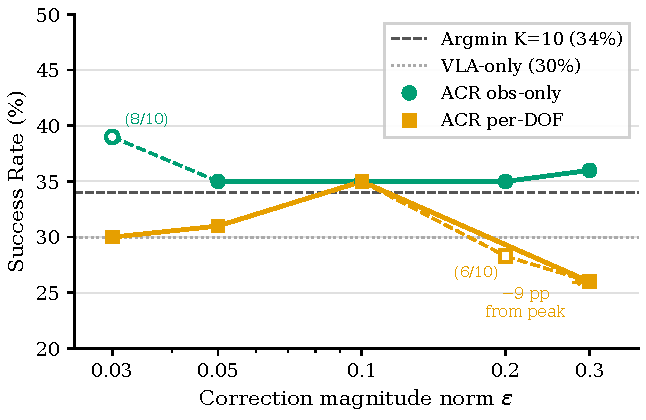
\includegraphics[width=\linewidth]{figures/fig3_magnitude_sweep.pdf}
\caption{Success rate (\%) on LIBERO-Spatial as a function of magnitude bound $\varepsilon$. obs\_only (solid teal) maintains 35--39\% across $\varepsilon \in [0.03, 0.3]$. perdof (solid orange) peaks at $\varepsilon{=}0.1$ (35\%) and collapses to 26\% at $\varepsilon{=}0.3$ ($-$9\,pp). Dashed segments indicate partial data ($<$10 tasks). The Argmin baseline (dashed gray, 34\%) is independent of $\varepsilon$.}
\label{fig:magnitude}
\end{figure}

\begin{table}[t]
\centering
\caption{Success rate (\%) on LIBERO-Spatial across magnitude bounds $\varepsilon$. The Argmin baseline (34\%, no correction) is independent of $\varepsilon$.}
\label{tab:magnitude}
\small
\begin{tabular}{lcccc}
\toprule
$\varepsilon$ & 0.05 & 0.1 & 0.3 & 1.42 \\
\midrule
obs\_only & 35.0 & 35.0 & 36.0 & --- \\
perdof    & 31.0 & 35.0 & 26.0 & 0.0 \\
\midrule
Argmin (ref.) & \multicolumn{4}{c}{34.0 (flat, no correction)} \\
\bottomrule
\end{tabular}
\end{table}

\paragraph{obs\_only is robust.}
The obs\_only variant maintains 35--36\% across the full range $\varepsilon \in [0.05, 0.3]$---a remarkably flat profile.
This stability means the practitioner need not carefully tune $\varepsilon$; any value in $[0.05, 0.2]$ yields near-identical performance.

\paragraph{perdof is fragile.}
In contrast, perdof peaks at 35\% when $\varepsilon{=}0.1$ but collapses to 26\% at $\varepsilon{=}0.3$---a 9\,pp drop.
This fragility suggests that the noisy conformal features cause the CRM to predict unreliable correction directions; when the magnitude bound is loose enough to accommodate these directions, performance degrades.
At $\varepsilon{=}0.1$, the tight bound masks the problem by clipping erroneous corrections.

\paragraph{Unbounded correction is catastrophic.}
Without magnitude control ($\varepsilon{\approx}1.42$, the natural CRM output norm), perdof achieves 0\% on LIBERO-Spatial---compounding error across the trajectory destroys performance entirely (Section~\ref{sec:magnitude}).
The Argmin baseline (34\%) outperforms all CRM variants at this setting, demonstrating that unbounded correction is harmful.
The obs\_only variant was not evaluated at $\varepsilon{=}1.42$ on spatial, though analogous catastrophic failure is expected given the magnitude of unconstrained corrections.

\paragraph{Practical recommendation.}
The safe operating range is $\varepsilon \in [0.05, 0.2]$.
Within this range, obs\_only is the only variant that consistently matches or exceeds the Argmin baseline.
We use $\varepsilon{=}0.1$ as the default, which provides a conservative margin below the point where perdof begins to degrade.


\subsection{Per-Task Analysis}
\label{sec:per_task}

Per-task success rate breakdowns will reveal which task categories benefit most from residual correction and where the method provides no improvement.

[\textsc{pending}: seed43] --- A per-task heatmap comparing obs\_only, Argmin, and VLA-only across all 20 tasks (10 LIBERO-Spatial + 10 LIBERO-Object) will be included upon completion of the seed 43 replication.
We expect the analysis to show that obs\_only's gains on LIBERO-Object concentrate on tasks requiring precise object grasping under visual variation, while LIBERO-Spatial tasks remain uniformly unaffected by correction.
Task difficulty analysis (measured by VLA-only success rate) will additionally test whether CRM helps more on medium-difficulty tasks where the base policy partially succeeds, versus easy tasks (ceiling effect) or hard tasks (base policy too far from success for small corrections to recover).
